\documentclass[12pt]{article}
\usepackage{amsmath}
\usepackage{graphicx}
\usepackage{hyperref}
\usepackage{listings}
\usepackage{color}

\title{Operating System Course Report - First Half of the Semester}
\author{B class}
\date{\today}
\begin{document}
	
	\maketitle
	\newpage
	
	\tableofcontents
	\newpage
	
	\section{Introduction}
	This report summarizes the topics covered during the first half of the Operating System course. It includes theoretical concepts, practical implementations, and assignments. The course focuses on the fundamentals of operating systems, including system architecture, process management, CPU scheduling, and deadlock handling.
	
	\section{Course Overview}
	\subsection{Objectives}
	The main objectives of this course are:
	\begin{itemize}
		\item To understand the basic components and architecture of a computer system.
		\item To learn process management, scheduling, and inter-process communication.
		\item To explore file systems, input/output management, and virtualization.
		\item To study the prevention and handling of deadlocks in operating systems.
	\end{itemize}
	
	\subsection{Course Structure}
	The course is divided into two halves. This report focuses on the first half, which covers:
	\begin{itemize}
		\item Basic Concepts and Components of Computer Systems
		\item System Performance and Metrics
		\item System Architecture of Computer Systems
		\item Process Description and Control
		\item Scheduling Algorithms
		\item Process Creation and Termination
		\item Introduction to Threads
		\item File Systems
		\item Input and Output Management
		\item Deadlock Introduction and Prevention
		\item User Interface Management
		\item Virtualization in Operating Systems
	\end{itemize}
	
	\section{Topics Covered}
	
	\subsection{Basic Concepts and Components of Computer Systems}
	This section explains the fundamental components that make up a computer system, including the CPU, memory, storage, and input/output devices.
	
	\subsection{System Performance and Metrics}
	This section introduces various system performance metrics used to measure the efficiency of a computer system, including throughput, response time, and utilization.
	
	\subsection{System Architecture of Computer Systems}
	\begin{figure}[h]
		\centering
		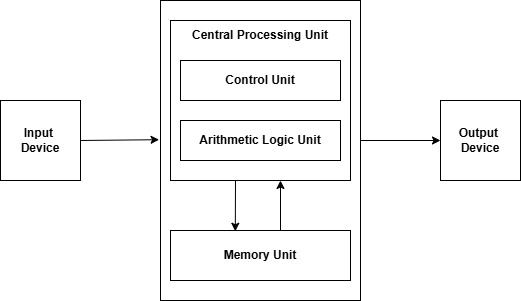
\includegraphics[width=0.5\textwidth]{asset/arsitektur von neumann.jpg}
		\caption{Arsitektur Von Neumann} 
		\label{fig:contoh_gambar} % Menambahkan label untuk referensi silang
	\end{figure}
	\subsubsection{Arsitektur Komputer}
	Arsitektur komputer merujuk pada struktur dasar dari sistem komputer yang melibatkan perangkat keras atau \textit{hardware} dan perangkat lunak atau \textit{software} yang bekerja sama untuk menjalankan instruksi dan memproses data. Arsitektur komputer lebih menekankan fokus pada konsep dan prinsip dasar yang mengatur operasi komputer secara umum. Berikut ini merupakan komponen utama dari arsitektur komputer.
	\subsubsection*{\textit{Control Unit}}
	\textit{Control Unit} merupakan pusat dari otak komputer. \textit{Control Unit} bertugas untuk mengawasi berbagai siklus instruksi sehingga dapat melakukan \textit{control} pada sinyal-sinyal yang relevan pada saat yang tepat, supaya operasi \textit{micro} dapat dikerjakan pada CPU dan unit eksternal yang terhubung pada 
	CPU seperti \textit{memory} dan \textit{input output devices} atau \textit{contoller}.
	\textit{Control unit} dirancang pada suatu data spesifik yang berada pada organisasi \textit{datapath} ALU (unit logika aritmatika), register serta sebagainya yang berada pada CPU.
	\subsubsection*{\textit{Arithmetic Logic Unit}}
	Semua komponen CPU yang lainnya dan seluruh komponen penyusun komputer membawa data ke ALU untuk diproses dan mengambil kembali hasil setelah diproses ALU. ALU membentuk fungsi-fungsi pengolahan data pada komputer, di antaranya operasi aritmatika dan logika terhadap data. Adapun tugas ALU yaitu melakukan perintah yang berhubungan dengan perhitungan aritmatika serta mengambil keputusan dari suatu operasi sesuai dengan instruksi dari program yang disebut operasi logika. Karena itu, ALU berguna untuk melakukan proses data dalam bentuk angka dan logika.
	\subsubsection*{Memori}
	Memori adalah tempat penyimpanan informasi yang dapat diakses oleh CPU. Sistem komputer modern menggunakan beberapa jenis memori, masing-masing dengan tujuan dan karakteristiknya sendiri. 
	\begin{itemize}
		\item RAM (\textit{Random Access Memory}) adalah jenis memori yang digunakan oleh komputer untuk menyimpan data sementara yang dibutuhkan CPU saat menjalankan program atau tugas tertentu. Keuntungan RAM adalah kecepatan akses tinggi, tetapi data yang disimpan di dalamnya hilang ketika daya listrik dimatikan
		\item ROM (\textit{Read Only Memory}) adalah jenis memori yang menyimpan data yang tidak berubah, bahkan ketika daya listrik dimatikan. 
	\end{itemize}
	\subsubsection*{Input/Output}
	Input/Output (I/O) merupakan bagian dari sebuah sistem mikroprosesor yang berfungsi untuk dapat berinteraksi dengan berbagai \textit{peripheral} perangkat luar. Unit input merupakan unit luar yang berfungsi sebagai unit yang dapat memberikan sebuah instruksi atau memasukan sebuah data dari perangkat eksternal ke dalam mikroprosesor, sebagai Contoh dari unit input adalah sebuah data yang bersumber dari perangkat input berupa \textit{keyboard} atau \textit{mouse}. Sedangkan unit output adalah sebuah unit yang berfungsi untuk dapat menampilkan sebuah data yang dikirimkan dari  mikroprosesor, sebagai Contoh dari unit output adalah sebuah hasil pengolahan data yang dapat diterjemahkan oleh pengguna baik berupa gambar, suara, visual atau hasil cetak yaitu berupa monitor, \textit{printer} atau \textit{sound audio}.
	
	\begin{thebibliography}{widestlabel}
		\bibitem{Cahyaningrum2023}
		Cahyaningrum, Y. Y. (2023). \textit{ARISTEKTUR DAN ORGANISASI KOMPUTER}. Yogyakarta: PT Penamuda Media.
		\bibitem{Amrival2013}
		Amrival, V. A. (2013). \textit{ARSITEKTUR KOMPUTER: Teori dan Perkembangannya}. Jakarta: Halaman Moeka Publishing.
	\end{thebibliography}
	
	\subsection{Process Description and Control}
	Processes are a central concept in operating systems. This section covers:
	\begin{itemize}
		\item Process states and state transitions
		\item Process control block (PCB)
		\item Context switching
	\end{itemize}
	
	\subsection{Scheduling Algorithms}
	This section covers:
	\begin{itemize}
		\item First-Come, First-Served (FCFS)
		\item Shortest Job Next (SJN)
		\item Round Robin (RR)
	\end{itemize}
	It explains how these algorithms are used to allocate CPU time to processes.
	
	\subsection{Process Creation and Termination}
	Details how processes are created and terminated by the operating system, including:
	\begin{itemize}
		\item Process spawning
		\item Process termination conditions
	\end{itemize}
	
	\subsection{Introduction to Threads}
	This section introduces the concept of threads and their relation to processes, covering:
	\begin{itemize}
		\item Single-threaded vs. multi-threaded processes
		\item Benefits of multithreading
	\end{itemize}
	
	\subsection{File Systems}
	File systems provide a way for the operating system to store, retrieve, and manage data. This section explains:
	\begin{itemize}
		\item File system structure
		\item File access methods
		\item Directory management
	\end{itemize}
	
	\subsection{Input and Output Management}
	Input and output management is key for handling the interaction between the system and external devices. This section includes:
	\begin{itemize}
		\item Device drivers
		\item I/O scheduling
	\end{itemize}
	
	\subsection{Deadlock Introduction and Prevention}
	Explores the concept of deadlocks and methods for preventing them:
	\begin{itemize}
		\item Deadlock conditions
		\item Deadlock prevention techniques
	\end{itemize}
	
	\subsection{User Interface Management}
	This section discusses the role of the operating system in managing the user interface. Topics covered include:
	\begin{itemize}
		\item Graphical User Interface (GUI)
		\item Command-Line Interface (CLI)
		\item Interaction between the user and the operating system
	\end{itemize}
	
	\subsection{Virtualization in Operating Systems}
	Virtualization allows multiple operating systems to run concurrently on a single physical machine. This section explores:
	\begin{itemize}
		\item Concept of virtualization
		\item Hypervisors and their types
		\item Benefits of virtualization in modern computing
	\end{itemize}
	
	\section{Assignments and Practical Work}
	\subsection{Assignment 1: Process Scheduling}
	Students were tasked with implementing various process scheduling algorithms (e.g., FCFS, SJN, and RR) and comparing their performance under different conditions.
	
	\subsection{Assignment 2: Deadlock Handling}
	In this assignment, students were asked to simulate different deadlock scenarios and explore various prevention methods.
	
	\subsection{Assignment 3: Multithreading and Amdahl's Law}
	This assignment involved designing a multithreading scenario to solve a computationally intensive problem. Students then applied *Amdahl's Law* to calculate the theoretical speedup of the program as the number of threads increased.
	
	\subsection{Assignment 4: Simple Command-Line Interface (CLI) for User Interface Management}
	Students were tasked with creating a simple *CLI* for user interface management. The CLI should support basic commands such as file manipulation (creating, listing, and deleting files), process management, and system status reporting.
	
	Soal:
	\par Buatlah program CLI sederhana yang memungkinkan pengguna untuk mengelola tampilan antarmuka pengguna (UI). Program ini harus memberikan opsi untuk menampilkan menu, menambahkan item ke UI, dan menghapus item dari UI.
	Program harus memiliki opsi sebagai berikut:
	\begin{itemize}
		
		\item Tampilkan item dalam UI
		\item Tambah item ke UI
		\item Hapus item dari UI
		\item Keluar
	\end{itemize}
	\par Implementasikan program dalam Python menggunakan konsep CLI.
	
	\lstset{ 
		language=Python, % Bahasa pemrograman
		backgroundcolor=\color{white}, % Warna latar belakang
		commentstyle=\color{gray}, % Warna komentar
		keywordstyle=\color{blue}, % Warna string
		basicstyle=\ttfamily\footnotesize, % Gaya dasar teks
		breaklines=true,  % Otomatis break baris
		frame=single, % Garis kotak di sekitar kode
		showstringspaces=false, % Hilangkan spasi dalam string
	}
	
	\begin{lstlisting}
		def display_menu():
		print("=== UI Management ===")
		print("1. Tampilkan item dalam UI")
		print("2. Tambah item ke UI")
		print("3. Hapus item dari UI")
		print("4. Keluar")
		
		def display_ui(ui_items):
		if ui_items:
		print("\nItem UI saat ini:")
		for idx, item in enumerate(ui_items, start=1):
		print(f"{idx}. {item}")
		else:
		print("\nUI masih kosong.")
		print()
		
		def add_ui_item(ui_items):
		item = input("Masukkan nama item yang ingin ditambahkan ke UI: ")
		ui_items.append(item)
		print(f"'{item}' berhasil ditambahkan ke UI.\n")
		
		def remove_ui_item(ui_items):
		if not ui_items:
		print("\nUI kosong, tidak ada item yang bisa dihapus.\n")
		return
		display_ui(ui_items)
		try:
		idx = int(input("Masukkan nomor item yang ingin dihapus: "))
		if 1 <= idx <= len(ui_items):
		removed_item = ui_items.pop(idx - 1)
		print(f"'{removed_item}' berhasil dihapus dari UI.\n")
		else:
		print("Nomor item tidak valid.\n")
		except ValueError:
		print("Input tidak valid, masukkan angka.\n")
		
		def cli_ui_management():
		ui_items = []
		while True:
		display_menu()
		try:
		choice = int(input("Pilih opsi: "))
		if choice == 1:
		display_ui(ui_items)
		elif choice == 2:
		add_ui_item(ui_items)
		elif choice == 3:
		remove_ui_item(ui_items)
		elif choice == 4:
		print("Keluar dari program.")
		break
		else:
		print("Pilihan tidak valid, coba lagi.\n")
		except ValueError:
		print("Input tidak valid, masukkan angka.\n")
		
		
		if __name__ == "__main__":
		cli_ui_management()
		
	\end{lstlisting}
	
	
	\subsection{Assignment 5: File System Access}
	In this assignment, students implemented file system access routines, including:
	\begin{itemize}
		\item File creation and deletion
		\item Reading from and writing to files
		\item Navigating directories and managing file permissions
	\end{itemize}
	
	Soal: 
	\par Buatlah program Python yang melakukan operasi dasar pada sistem file. Program ini harus:
	\begin{itemize}
		\item Membaca isi dari file tertentu
		\item Menambahkan teks ke dalam file
		\item Menampilkan daftar file dalam direktori
	\end{itemize}
	 Implementasikan program dalam Python menggunakan konsep CLI.
	 
	 \lstset{ 
	 	language=Python, % Bahasa pemrograman
	 	backgroundcolor=\color{white}, % Warna latar belakang
	 	commentstyle=\color{gray}, % Warna komentar
	 	keywordstyle=\color{blue}, % Warna string
	 	basicstyle=\ttfamily\footnotesize, % Gaya dasar teks
	 	breaklines=true,  % Otomatis break baris
	 	frame=single, % Garis kotak di sekitar kode
	 	showstringspaces=false, % Hilangkan spasi dalam string
	 }
	 
	 \begin{lstlisting}
	 	import os
	 	
	 	def list_files_in_directory(directory):
	 	try:
	 	files = os.listdir(directory)
	 	print(f"\nDaftar file dalam direktori '{directory}':")
	 	for file in files:
	 	print(file)
	 	print()
	 	except FileNotFoundError:
	 	print(f"Direktori '{directory}' tidak ditemukan.\n")
	 	
	 	def read_file(file_path):
	 	try:
	 	with open(file_path, 'r') as file:
	 	content = file.read()
	 	print(f"\nIsi file '{file_path}':")
	 	print(content)
	 	print()
	 	except FileNotFoundError:
	 	print(f"File '{file_path}' tidak ditemukan.\n")
	 	except IOError:
	 	print(f"Tidak dapat membaca file '{file_path}'.\n")
	 	
	 	def write_to_file(file_path, text):
	 	try:
	 	with open(file_path, 'a') as file:
	 	file.write(text + "\n")
	 	print(f"Teks berhasil ditambahkan ke file '{file_path}'.\n")
	 	except IOError:
	 	print(f"Tidak dapat menulis ke file '{file_path}'.\n")
	 	
	 	def file_system_access():
	 	while True:
	 	print("=== File System Access ===")
	 	print("1. Tampilkan daftar file dalam direktori")
	 	print("2. Baca file")
	 	print("3. Tambah teks ke file")
	 	print("4. Keluar")
	 	
	 	try:
	 	choice = int(input("Pilih opsi: "))
	 	if choice == 1:
	 	directory = input("Masukkan direktori: ")
	 	list_files_in_directory(directory)
	 	elif choice == 2:
	 	file_path = input("Masukkan path file: ")
	 	read_file(file_path)
	 	elif choice == 3:
	 	file_path = input("Masukkan path file: ")
	 	text = input("Masukkan teks yang ingin ditambahkan: ")
	 	write_to_file(file_path, text)
	 	elif choice == 4:
	 	print("Keluar dari program.")
	 	break
	 	else:
	 	print("Pilihan tidak valid, coba lagi.\n")
	 	except ValueError:
	 	print("Input tidak valid, masukkan angka.\n")
	 	
	 	if __name__ == "__main__":
	 	file_system_access()
	 \end{lstlisting}
	
	\section{Conclusion}
	The first half of the course introduced core operating system concepts, including process management, scheduling, multithreading, and file system access. These topics provided a foundation for more advanced topics to be covered in the second half of the course.
	
\end{document}